% Options for packages loaded elsewhere
\PassOptionsToPackage{unicode}{hyperref}
\PassOptionsToPackage{hyphens}{url}
\documentclass[
  ignorenonframetext,
]{beamer}
\newif\ifbibliography
\usepackage{pgfpages}
\setbeamertemplate{caption}[numbered]
\setbeamertemplate{caption label separator}{: }
\setbeamercolor{caption name}{fg=normal text.fg}
\beamertemplatenavigationsymbolsempty
% remove section numbering
\setbeamertemplate{part page}{
  \centering
  \begin{beamercolorbox}[sep=16pt,center]{part title}
    \usebeamerfont{part title}\insertpart\par
  \end{beamercolorbox}
}
\setbeamertemplate{section page}{
  \centering
  \begin{beamercolorbox}[sep=12pt,center]{section title}
    \usebeamerfont{section title}\insertsection\par
  \end{beamercolorbox}
}
\setbeamertemplate{subsection page}{
  \centering
  \begin{beamercolorbox}[sep=8pt,center]{subsection title}
    \usebeamerfont{subsection title}\insertsubsection\par
  \end{beamercolorbox}
}
% Prevent slide breaks in the middle of a paragraph
\widowpenalties 1 10000
\raggedbottom
\AtBeginPart{
  \frame{\partpage}
}
\AtBeginSection{
  \ifbibliography
  \else
    \frame{\sectionpage}
  \fi
}
\AtBeginSubsection{
  \frame{\subsectionpage}
}
\usepackage{iftex}
\ifPDFTeX
  \usepackage[T1]{fontenc}
  \usepackage[utf8]{inputenc}
  \usepackage{textcomp} % provide euro and other symbols
\else % if luatex or xetex
  \usepackage{unicode-math} % this also loads fontspec
  \defaultfontfeatures{Scale=MatchLowercase}
  \defaultfontfeatures[\rmfamily]{Ligatures=TeX,Scale=1}
\fi
\usepackage{lmodern}
\usetheme[]{Montpellier}
\ifPDFTeX\else
  % xetex/luatex font selection
\fi
% Use upquote if available, for straight quotes in verbatim environments
\IfFileExists{upquote.sty}{\usepackage{upquote}}{}
\IfFileExists{microtype.sty}{% use microtype if available
  \usepackage[]{microtype}
  \UseMicrotypeSet[protrusion]{basicmath} % disable protrusion for tt fonts
}{}
\makeatletter
\@ifundefined{KOMAClassName}{% if non-KOMA class
  \IfFileExists{parskip.sty}{%
    \usepackage{parskip}
  }{% else
    \setlength{\parindent}{0pt}
    \setlength{\parskip}{6pt plus 2pt minus 1pt}}
}{% if KOMA class
  \KOMAoptions{parskip=half}}
\makeatother
\usepackage{color}
\usepackage{fancyvrb}
\newcommand{\VerbBar}{|}
\newcommand{\VERB}{\Verb[commandchars=\\\{\}]}
\DefineVerbatimEnvironment{Highlighting}{Verbatim}{commandchars=\\\{\}}
% Add ',fontsize=\small' for more characters per line
\usepackage{framed}
\definecolor{shadecolor}{RGB}{248,248,248}
\newenvironment{Shaded}{\begin{snugshade}}{\end{snugshade}}
\newcommand{\AlertTok}[1]{\textcolor[rgb]{0.94,0.16,0.16}{#1}}
\newcommand{\AnnotationTok}[1]{\textcolor[rgb]{0.56,0.35,0.01}{\textbf{\textit{#1}}}}
\newcommand{\AttributeTok}[1]{\textcolor[rgb]{0.13,0.29,0.53}{#1}}
\newcommand{\BaseNTok}[1]{\textcolor[rgb]{0.00,0.00,0.81}{#1}}
\newcommand{\BuiltInTok}[1]{#1}
\newcommand{\CharTok}[1]{\textcolor[rgb]{0.31,0.60,0.02}{#1}}
\newcommand{\CommentTok}[1]{\textcolor[rgb]{0.56,0.35,0.01}{\textit{#1}}}
\newcommand{\CommentVarTok}[1]{\textcolor[rgb]{0.56,0.35,0.01}{\textbf{\textit{#1}}}}
\newcommand{\ConstantTok}[1]{\textcolor[rgb]{0.56,0.35,0.01}{#1}}
\newcommand{\ControlFlowTok}[1]{\textcolor[rgb]{0.13,0.29,0.53}{\textbf{#1}}}
\newcommand{\DataTypeTok}[1]{\textcolor[rgb]{0.13,0.29,0.53}{#1}}
\newcommand{\DecValTok}[1]{\textcolor[rgb]{0.00,0.00,0.81}{#1}}
\newcommand{\DocumentationTok}[1]{\textcolor[rgb]{0.56,0.35,0.01}{\textbf{\textit{#1}}}}
\newcommand{\ErrorTok}[1]{\textcolor[rgb]{0.64,0.00,0.00}{\textbf{#1}}}
\newcommand{\ExtensionTok}[1]{#1}
\newcommand{\FloatTok}[1]{\textcolor[rgb]{0.00,0.00,0.81}{#1}}
\newcommand{\FunctionTok}[1]{\textcolor[rgb]{0.13,0.29,0.53}{\textbf{#1}}}
\newcommand{\ImportTok}[1]{#1}
\newcommand{\InformationTok}[1]{\textcolor[rgb]{0.56,0.35,0.01}{\textbf{\textit{#1}}}}
\newcommand{\KeywordTok}[1]{\textcolor[rgb]{0.13,0.29,0.53}{\textbf{#1}}}
\newcommand{\NormalTok}[1]{#1}
\newcommand{\OperatorTok}[1]{\textcolor[rgb]{0.81,0.36,0.00}{\textbf{#1}}}
\newcommand{\OtherTok}[1]{\textcolor[rgb]{0.56,0.35,0.01}{#1}}
\newcommand{\PreprocessorTok}[1]{\textcolor[rgb]{0.56,0.35,0.01}{\textit{#1}}}
\newcommand{\RegionMarkerTok}[1]{#1}
\newcommand{\SpecialCharTok}[1]{\textcolor[rgb]{0.81,0.36,0.00}{\textbf{#1}}}
\newcommand{\SpecialStringTok}[1]{\textcolor[rgb]{0.31,0.60,0.02}{#1}}
\newcommand{\StringTok}[1]{\textcolor[rgb]{0.31,0.60,0.02}{#1}}
\newcommand{\VariableTok}[1]{\textcolor[rgb]{0.00,0.00,0.00}{#1}}
\newcommand{\VerbatimStringTok}[1]{\textcolor[rgb]{0.31,0.60,0.02}{#1}}
\newcommand{\WarningTok}[1]{\textcolor[rgb]{0.56,0.35,0.01}{\textbf{\textit{#1}}}}
\setlength{\emergencystretch}{3em} % prevent overfull lines
\providecommand{\tightlist}{%
  \setlength{\itemsep}{0pt}\setlength{\parskip}{0pt}}
%\documentclass[unicode,10pt]{beamer}% 'unicode'が必要
\usepackage{luatexja}% 日本語を使う場合は必須
%\usepackage[japanese]{babel}	
%\usefonttheme[onlymath]{serif}
%\usepackage[T1]{fontenc} %これを使うと、ギリシャ文字が出ない
%\usepackage{textcomp}
%\usepackage[scale=1.0]{tgheros} % Sans serif font
%\usepackage[scaled]{beramono} % Monospace font
%\usepackage{luatexja-otf}
%\renewcommand{\kanjifamilydefault}{\gtdefault}
%\usepackage[haranoaji]{luatexja-preset}

% スライド番号の表示 %%%%%%%%%%%%%%%%%%%
\makeatletter
\setbeamertemplate{footline}{%
  \leavevmode%
  \hbox{%
  \begin{beamercolorbox}[wd=.5\paperwidth,ht=2.25ex,dp=1ex,right]{date in head/foot}%
    \insertframenumber{} \hspace*{2ex} % new version without total frames
  \end{beamercolorbox}}%
  \vskip0pt%
}
\makeatother
% スライド番号の表示 %%%%%%%%%%%%%%%%%%%
\usepackage{bookmark}
\IfFileExists{xurl.sty}{\usepackage{xurl}}{} % add URL line breaks if available
\urlstyle{same}
\hypersetup{
  hidelinks,
  pdfcreator={LaTeX via pandoc}}

\title{第6章: 確率}
\subtitle{Elena Llaudet \& Kosuke Imai.\\
Data Analysis for Social Science: A Friendly and Practical
Introduction.}
\author{}
\date{\vspace{-2.5em}2026-03-09}

\begin{document}
\frame{\titlepage}

\section{6.1 確率の重要性}\label{ux78baux7387ux306eux91cdux8981ux6027}

\begin{frame}{なぜ確率を学ぶのか？}
\phantomsection\label{ux306aux305cux78baux7387ux3092ux5b66ux3076ux306eux304b}
\begin{itemize}
\tightlist
\item
  データ分析には常に\textbf{不確実性} (Uncertainty) が伴う。
\item
  標本から母集団を推測する際、その推測がどれくらい正確かを評価するために確率の知識が必要。
\item
  社会科学における例：

  \begin{itemize}
  \tightlist
  \item
    世論調査の誤差の評価
  \item
    政策効果が偶然ではないことの確認
  \item
    将来の出来事の発生予測
  \end{itemize}
\end{itemize}
\end{frame}

\section{6.2
ベルヌーイ分布}\label{ux30d9ux30ebux30ccux30fcux30a4ux5206ux5e03}

\begin{frame}[fragile]{ベルヌーイ分布 (Bernoulli Distribution)}
\phantomsection\label{ux30d9ux30ebux30ccux30fcux30a4ux5206ux5e03-bernoulli-distribution}
\begin{itemize}
\tightlist
\item
  2つの結果（成功/失敗、1/0）しかない試行の確率分布。
\item
  例：コイン投げ（表=1, 裏=0）
\end{itemize}

\footnotesize

\begin{Shaded}
\begin{Highlighting}[]
\CommentTok{\# 100万回のコイン投げシミュレーション}
\NormalTok{possible\_values }\OtherTok{\textless{}{-}} \FunctionTok{c}\NormalTok{(}\DecValTok{1}\NormalTok{, }\DecValTok{0}\NormalTok{)}
\NormalTok{flips }\OtherTok{\textless{}{-}} \FunctionTok{sample}\NormalTok{(possible\_values, }\AttributeTok{size =} \DecValTok{1000000}\NormalTok{, }
                \AttributeTok{replace =} \ConstantTok{TRUE}\NormalTok{, }\AttributeTok{prob =} \FunctionTok{c}\NormalTok{(}\FloatTok{0.5}\NormalTok{, }\FloatTok{0.5}\NormalTok{))}

\CommentTok{\# 比率の確認}
\FunctionTok{prop.table}\NormalTok{(}\FunctionTok{table}\NormalTok{(flips))}
\end{Highlighting}
\end{Shaded}

\begin{verbatim}
## flips
##        0        1 
## 0.500061 0.499939
\end{verbatim}

\begin{Shaded}
\begin{Highlighting}[]
\CommentTok{\# 平均（期待値）}
\FunctionTok{mean}\NormalTok{(flips)}
\end{Highlighting}
\end{Shaded}

\begin{verbatim}
## [1] 0.499939
\end{verbatim}

\normalsize
\end{frame}

\section{6.3 正規分布}\label{ux6b63ux898fux5206ux5e03}

\begin{frame}[fragile]{正規分布 (Normal Distribution)}
\phantomsection\label{ux6b63ux898fux5206ux5e03-normal-distribution}
\begin{itemize}
\tightlist
\item
  左右対称の釣鐘型の分布。多くの自然・社会現象に現れる。
\item
  平均 (\(\mu\)) と標準偏差 (\(\sigma\)) で形状が決まる。
\end{itemize}

\footnotesize

\begin{Shaded}
\begin{Highlighting}[]
\CommentTok{\# STARデータの読み込み}
\NormalTok{star }\OtherTok{\textless{}{-}} \FunctionTok{read.csv}\NormalTok{(}\StringTok{"STAR.csv"}\NormalTok{)}
\CommentTok{\# 読解力テストの得点分布}
\FunctionTok{hist}\NormalTok{(star}\SpecialCharTok{$}\NormalTok{reading, }\AttributeTok{freq =} \ConstantTok{FALSE}\NormalTok{, }
     \AttributeTok{main =} \StringTok{"Histogram of Reading Scores"}\NormalTok{, }
     \AttributeTok{xlab =} \StringTok{"Reading Score"}\NormalTok{)}
\end{Highlighting}
\end{Shaded}

\begin{center}
\includegraphics[height=0.4\textheight]{DSS_Ch06_files/figure-beamer/unnamed-chunk-2-1} \end{center}

\normalsize
\end{frame}

\begin{frame}[fragile]{標準正規分布 (Standard Normal Distribution)}
\phantomsection\label{ux6a19ux6e96ux6b63ux898fux5206ux5e03-standard-normal-distribution}
\begin{itemize}
\tightlist
\item
  平均 = 0, 標準偏差 = 1 の正規分布。
\item
  \texttt{pnorm()} 関数を用いて、ある値以下の確率を計算できる。
\end{itemize}

\begin{Shaded}
\begin{Highlighting}[]
\CommentTok{\# Z \textless{}= {-}1.96 となる確率（約2.5\%）}
\FunctionTok{pnorm}\NormalTok{(}\SpecialCharTok{{-}}\FloatTok{1.96}\NormalTok{)}
\end{Highlighting}
\end{Shaded}

\begin{verbatim}
## [1] 0.0249979
\end{verbatim}

\begin{Shaded}
\begin{Highlighting}[]
\CommentTok{\# {-}1.96 \textless{}= Z \textless{}= 1.96 となる確率（約95\%）}
\FunctionTok{pnorm}\NormalTok{(}\FloatTok{1.96}\NormalTok{) }\SpecialCharTok{{-}} \FunctionTok{pnorm}\NormalTok{(}\SpecialCharTok{{-}}\FloatTok{1.96}\NormalTok{)}
\end{Highlighting}
\end{Shaded}

\begin{verbatim}
## [1] 0.9500042
\end{verbatim}
\end{frame}

\section{6.4 大数の法則}\label{ux5927ux6570ux306eux6cd5ux5247}

\begin{frame}[fragile]{大数の法則 (Law of Large Numbers)}
\phantomsection\label{ux5927ux6570ux306eux6cd5ux5247-law-of-large-numbers}
\begin{itemize}
\tightlist
\item
  サンプルサイズ (\(n\)) が大きくなるほど、標本平均は母平均に近づく。
\end{itemize}

\scriptsize

\begin{Shaded}
\begin{Highlighting}[]
\CommentTok{\# 母集団の支持率 p = 0.6 とする}
\CommentTok{\# n = 10 の場合}
\FunctionTok{mean}\NormalTok{(}\FunctionTok{sample}\NormalTok{(}\FunctionTok{c}\NormalTok{(}\DecValTok{1}\NormalTok{, }\DecValTok{0}\NormalTok{), }\AttributeTok{size =} \DecValTok{10}\NormalTok{, }\AttributeTok{replace =} \ConstantTok{TRUE}\NormalTok{, }
            \AttributeTok{prob =} \FunctionTok{c}\NormalTok{(}\FloatTok{0.6}\NormalTok{, }\FloatTok{0.4}\NormalTok{)))}
\end{Highlighting}
\end{Shaded}

\begin{verbatim}
## [1] 0.7
\end{verbatim}

\begin{Shaded}
\begin{Highlighting}[]
\CommentTok{\# n = 1000 の場合}
\FunctionTok{mean}\NormalTok{(}\FunctionTok{sample}\NormalTok{(}\FunctionTok{c}\NormalTok{(}\DecValTok{1}\NormalTok{, }\DecValTok{0}\NormalTok{), }\AttributeTok{size =} \DecValTok{1000}\NormalTok{, }\AttributeTok{replace =} \ConstantTok{TRUE}\NormalTok{,}
            \AttributeTok{prob =} \FunctionTok{c}\NormalTok{(}\FloatTok{0.6}\NormalTok{, }\FloatTok{0.4}\NormalTok{)))}
\end{Highlighting}
\end{Shaded}

\begin{verbatim}
## [1] 0.59
\end{verbatim}

\begin{Shaded}
\begin{Highlighting}[]
\CommentTok{\# n = 1000000 の場合}
\FunctionTok{mean}\NormalTok{(}\FunctionTok{sample}\NormalTok{(}\FunctionTok{c}\NormalTok{(}\DecValTok{1}\NormalTok{, }\DecValTok{0}\NormalTok{), }\AttributeTok{size =} \DecValTok{1000000}\NormalTok{, }\AttributeTok{replace =} \ConstantTok{TRUE}\NormalTok{, }
            \AttributeTok{prob =} \FunctionTok{c}\NormalTok{(}\FloatTok{0.6}\NormalTok{, }\FloatTok{0.4}\NormalTok{)))}
\end{Highlighting}
\end{Shaded}

\begin{verbatim}
## [1] 0.600568
\end{verbatim}

\normalsize
\end{frame}

\section{6.5 中心極限定理}\label{ux4e2dux5fc3ux6975ux9650ux5b9aux7406}

\begin{frame}[fragile]{中心極限定理 (Central Limit Theorem)}
\phantomsection\label{ux4e2dux5fc3ux6975ux9650ux5b9aux7406-central-limit-theorem}
\begin{itemize}
\tightlist
\item
  もとの分布が何であれ、サンプルサイズが十分に大きければ、標本平均の分布は\textbf{正規分布}に近づく。
\item
  推測統計学の最も重要な基盤。
\end{itemize}

\footnotesize

\begin{Shaded}
\begin{Highlighting}[]
\CommentTok{\# シミュレーション：標本平均の分布}
\NormalTok{sample\_means }\OtherTok{\textless{}{-}} \FunctionTok{c}\NormalTok{()}
\ControlFlowTok{for}\NormalTok{(i }\ControlFlowTok{in} \DecValTok{1}\SpecialCharTok{:}\DecValTok{10000}\NormalTok{)\{}
\NormalTok{  sample\_means[i] }\OtherTok{\textless{}{-}} \FunctionTok{mean}\NormalTok{(}\FunctionTok{sample}\NormalTok{(}\FunctionTok{c}\NormalTok{(}\DecValTok{1}\NormalTok{, }\DecValTok{0}\NormalTok{), }
                                 \AttributeTok{size =} \DecValTok{1000}\NormalTok{, }
        \AttributeTok{replace =} \ConstantTok{TRUE}\NormalTok{, }\AttributeTok{prob =} \FunctionTok{c}\NormalTok{(}\FloatTok{0.6}\NormalTok{, }\FloatTok{0.4}\NormalTok{)))}
\NormalTok{\}}
\end{Highlighting}
\end{Shaded}

\normalsize
\end{frame}

\begin{frame}[fragile]{中心極限定理の視覚化}
\phantomsection\label{ux4e2dux5fc3ux6975ux9650ux5b9aux7406ux306eux8996ux899aux5316}
\footnotesize

\begin{Shaded}
\begin{Highlighting}[]
\FunctionTok{hist}\NormalTok{(sample\_means, }\AttributeTok{freq =} \ConstantTok{FALSE}\NormalTok{, }
     \AttributeTok{main =} \StringTok{"Distribution of Sample Means"}\NormalTok{, }
     \AttributeTok{xlab =} \StringTok{"Sample Mean"}\NormalTok{)}
\end{Highlighting}
\end{Shaded}

\begin{center}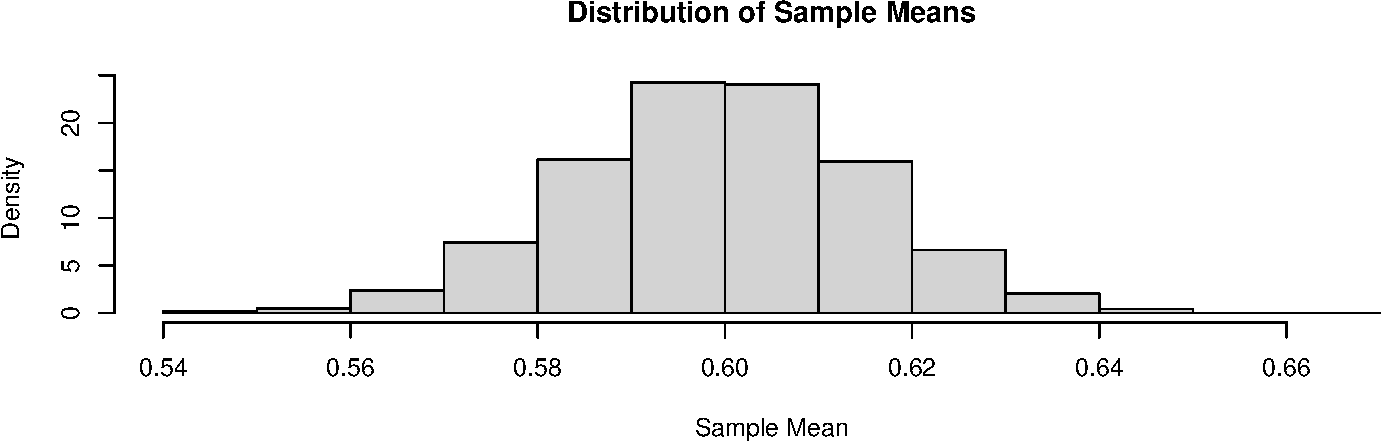
\includegraphics[height=0.4\textheight]{DSS_Ch06_files/figure-beamer/unnamed-chunk-6-1} \end{center}

\normalsize
\end{frame}

\section{6.6 まとめ}\label{ux307eux3068ux3081}

\begin{frame}{第6章のまとめ}
\phantomsection\label{ux7b2c6ux7ae0ux306eux307eux3068ux3081}
\begin{itemize}
\tightlist
\item
  \textbf{確率}は不確実性を数値化するための道具である。
\item
  \textbf{ベルヌーイ分布}は二値データを、\textbf{正規分布}は連続データをモデル化する。
\item
  \textbf{大数の法則}により、大きなサンプルはより正確な推測を可能にする。
\item
  \textbf{中心極限定理}により、標本平均の挙動を予測し、信頼区間や仮説検定に繋げることができる（次章）。
\end{itemize}
\end{frame}

\end{document}
